% D.19 梯形 ABCD，AD∥BC，AD=4，BC=10，E、F 是 AB、CD 中点，EF 交 AC、BD 于 M、N
\documentclass[tikz,border=4pt]{standalone}
\usepackage{ctex}
\usepackage{amsmath}
\usetikzlibrary{calc}
\begin{document}
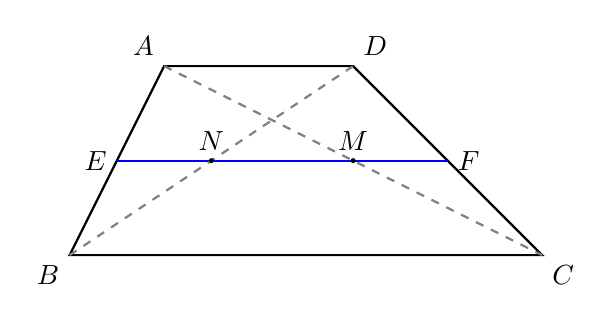
\begin{tikzpicture}[scale=0.6, thick]
  \coordinate (B) at (0, 0);
  \coordinate (C) at (10, 0);
  \coordinate (A) at (2, 4);
  \coordinate (D) at (6, 4);
  \coordinate (E) at ($(A)!0.5!(B)$);
  \coordinate (F) at ($(D)!0.5!(C)$);

  \draw (A) -- (B) -- (C) -- (D) -- cycle;
  \draw[blue] (E) -- (F);
  \draw[gray, dashed] (A) -- (C);
  \draw[gray, dashed] (B) -- (D);

  \coordinate (M) at (intersection of E--F and A--C);
  \coordinate (N) at (intersection of E--F and B--D);
  \fill (M) circle (1.5pt);
  \fill (N) circle (1.5pt);

  \node[above left]  at (A) {$A$};
  \node[below left]  at (B) {$B$};
  \node[below right] at (C) {$C$};
  \node[above right] at (D) {$D$};
  \node[left]        at (E) {$E$};
  \node[right]       at (F) {$F$};
  \node[above]       at (M) {$M$};
  \node[above]       at (N) {$N$};
\end{tikzpicture}
\end{document}
